\documentclass{article}
\usepackage{graphicx}
\usepackage[margin=1in]{geometry}
\usepackage[outdir=./]{epstopdf}  					% Avoids errors when input figures
\usepackage[labelsep=period,labelfont=bf]{caption}
%\usepackage{subcaption}
\usepackage{afterpage}

\begin{document}
	\afterpage{
	\begin{landscape}
		\begin{figure}[tbph]
			\caption{10-Year Synthetic Yields and Long-Horizon Implied Forecasts of the Short Rate} \label{fig:YLD10Y_CBP}
			\begin{center}								% center the minipage on the line
				\begin{minipage}{0.9\linewidth}
					\begin{center}							% center the figure inside the minipage
						\includegraphics[trim={0cm 0cm 0cm 0cm},clip,height=0.75\textheight,width=\linewidth]{../Figures/Data/YLD10Y_CBP.eps} \\
					\end{center}
					\fignotes{This figure plots the long-horizon implied forecast of the domestic nominal short-term interest rate (dashed line) and the 10-year synthetic yield (solid line). The implied forecast of the short rate is equal to the forecast of the U.S. real short-term interest rate corrected for a real forward premium plus the domestic consumer price inflation forecast, see text for details. The forecast of the U.S. real short-term rate is equal to the difference between the forecast of the three-month U.S. Treasury bill rate and the forecast of the U.S. consumer price inflation.}
				\end{minipage}
			\end{center}
		\end{figure}
	\end{landscape}
	}
\end{document}
% trim = {<left> <lower> <right> <upper>}